\newpage

\section{Diagrama de sequência}

Visto que a realização da autenticação e ativação de conta requer passos extras e regras a seguir, foi necessário criar diagramas de sequência para especificar a sequência de interações do cliente com o sistema.

\subsection{Diagrama de sequencia Login e ativação de conta}

Através deste diagrama (Figura~\ref{fig:29}) é entende-se que assim que o cliente deseja realizar o login, primeiramente tem de verificar as credenciais, caso estas se encontrem incorretas, este receberá uma mensagem de erro, caso as credenciais estejam válidas e a conta esteja ativada o cliente ficará autenticado. 

Caso o cliente coloque as credenciais corretas, mas a conta não esteja ativada, este irá realizar a ativação de conta, onde poderá enviar o código de ativação, caso esteja correto a sua conta será ativada, caso contrário este receberá uma mensagem de erro. O cliente poderá também cancelar a ativação de conta e pedir um novo email de ativação, onde será pedido novo código ao servidor, este será gerado e enviado para o cliente.

\begin{figure}[htb]
    \centering
    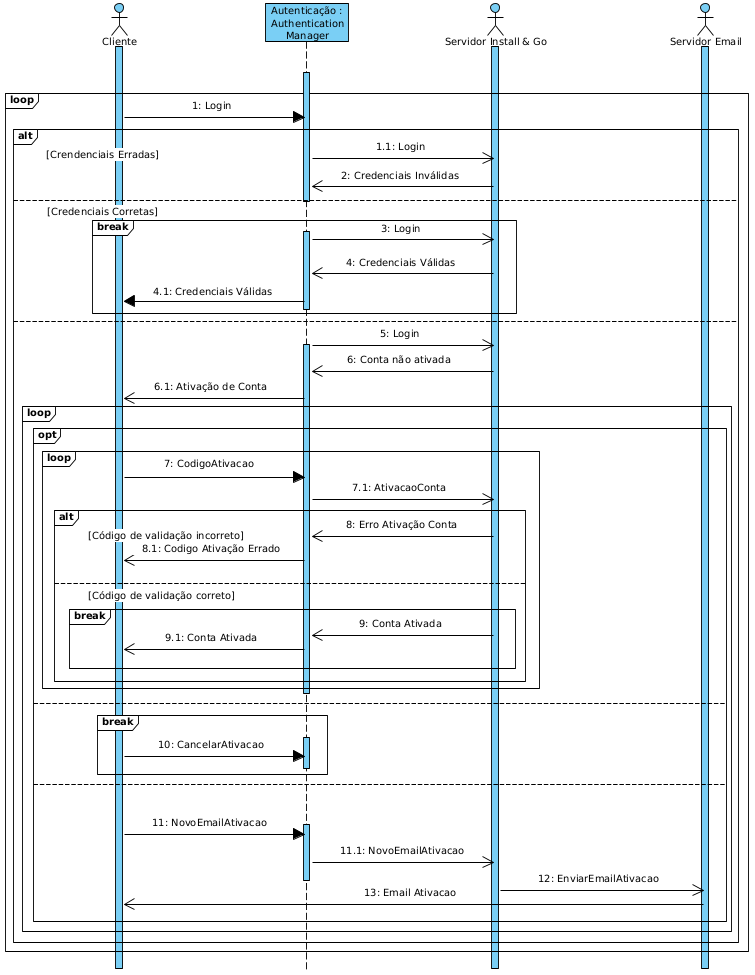
\includegraphics[width=0.67\textwidth]{images/diagramas/sequencia/diagrama_login.png}
    \caption{Diagrama de sequência de login e ativação de conta}
    \label{fig:30}
\end{figure}

\newpage

\subsection{Diagrama de sequencia Registo e ativação de conta}

Através do diagrama abaixo representado (Figura~\ref{fig30}) é possível perceber que quando o cliente realizar o registo este será enviado para o servidor, o qual registará o cliente com uma conta não ativada, para esta conta será gerado um código de ativação e enviado por email para o email de registo, após isto o cliente será encaminhado para a validação de conta, esta validação ocorre seguindo o mesmo processo mencionado no capítulo anterior.


\begin{figure}[htb]
    \centering
    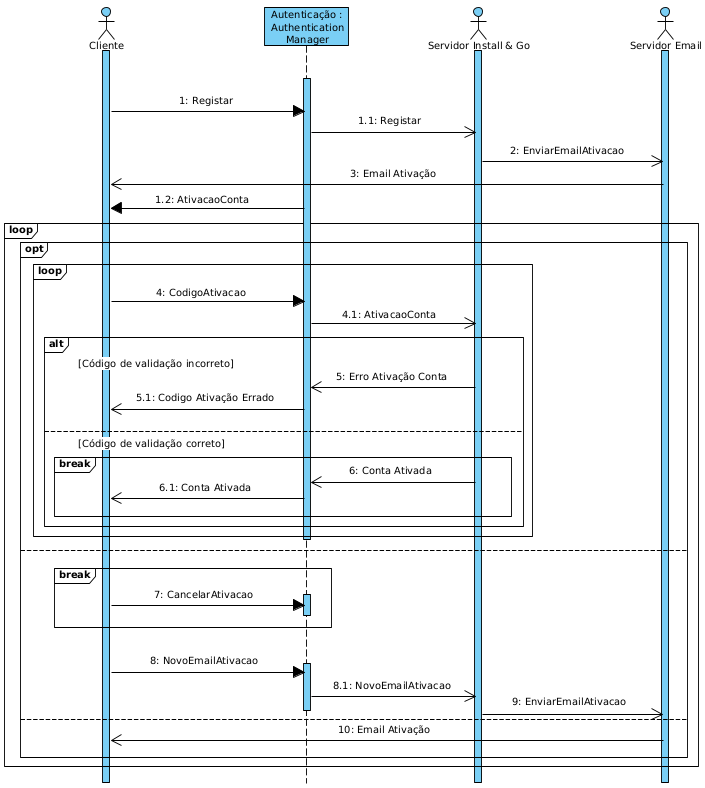
\includegraphics[width=0.8\textwidth]{images/diagramas/sequencia/diagrama_registo.png}
    \caption{Diagrama de sequência de registo e validação de conta}
    \label{fig:31}
\end{figure}